\documentclass{standalone}
\usepackage{graphicx}	
\usepackage{amssymb, amsmath, amsthm}
\usepackage{color}

\usepackage{tikz}
\usetikzlibrary{math, calc}

\definecolor{light}{RGB}{220, 188, 188}
\definecolor{mid}{RGB}{185, 124, 124}
\definecolor{dark}{RGB}{143, 39, 39}
\definecolor{highlight}{RGB}{180, 31, 180}
\definecolor{gray10}{gray}{0.1}
\definecolor{gray20}{gray}{0.2}
\definecolor{gray30}{gray}{0.3}
\definecolor{gray40}{gray}{0.4}
\definecolor{gray60}{gray}{0.6}
\definecolor{gray70}{gray}{0.7}
\definecolor{gray80}{gray}{0.8}
\definecolor{gray90}{gray}{0.9}
\definecolor{gray95}{gray}{0.95}
  
\newcommand\setcircbase[2]{{%
  \setbox0\hbox{%
    \raisebox{-0.5pt}{\scalebox{#2}{\Large$\bigcirc$}}}%
  \rlap{\hbox to \wd0{\hss$#1$\hss}}\box0%
}}

\newcommand\setcirc[1]{%
  \mathchoice%
    {\setcircbase{#1}{1.1}}% Display
    {\setcircbase{#1}{1.1}}% Text
    {\scriptsize\setcircbase{#1}{0.8}}% Subscript
    {\tiny\setcircbase{#1}{0.6}}% Subsubscript
}

\begin{document}

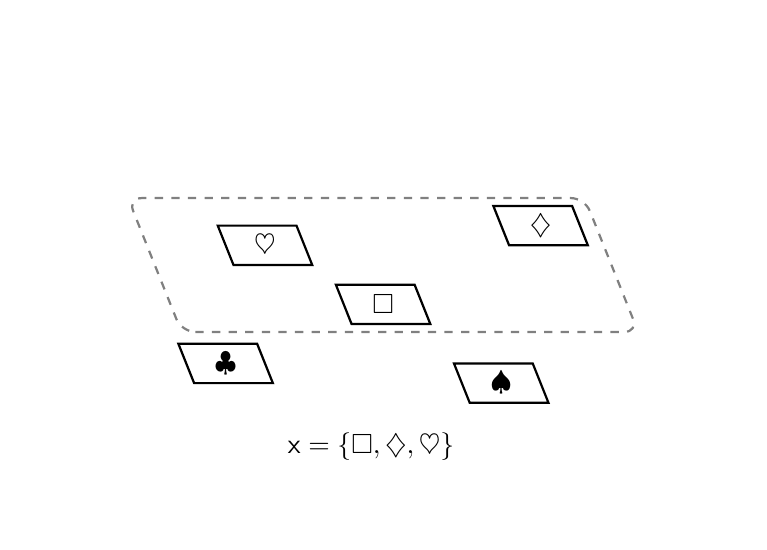
\begin{tikzpicture}[scale=1, thick]

  \draw[white] (-4.5, -2.75) rectangle (4.5, 3.5);
  
  \pgfmathsetmacro{\dx}{0.5}
  \pgfmathsetmacro{\dy}{0.25}
  \pgfmathsetmacro{\dz}{1}
  \pgfmathsetmacro{\tilt}{0.2}
  
  \foreach \x/\y\glyph [count=\n] in {0/0/\Box, -2/-0.75/\clubsuit, 2/1/\diamondsuit, 
                                      -1.5/0.75/\heartsuit, 1.5/-1/\spadesuit} {
    \begin{scope}[shift={(\x, \y)}]
      \node at (0, 0) { $\glyph$ };
      \draw[black]    ({-(1 - \tilt) * \dx}, -\dy) -- ({(1 + \tilt) * \dx}, -\dy) 
                   -- ({(1 - \tilt) * \dx}, \dy) -- ({-(1 + \tilt) * \dx}, \dy) -- cycle;
    \end{scope}
  }
  
  \pgfmathsetmacro{\dx}{2.9}
  \pgfmathsetmacro{\dy}{0.85}
  \pgfmathsetmacro{\tilt}{0.4 * \dy / \dx}
  \begin{scope}[shift={(0, 0.5)}]
    \draw[gray, dashed, rounded corners=5]    
         ({-(1 - \tilt) * \dx}, -\dy) -- ({+(1 + \tilt) * \dx}, -\dy) 
      -- ({+(1 - \tilt) * \dx}, +\dy) -- ({-(1 + \tilt) * \dx}, +\dy) 
      -- cycle;
  \end{scope}
  
  \node[black] at (-0.153, -1.8) { $\mathsf{x} = \{  \Box, \diamondsuit, \heartsuit  \}$ };
  
\end{tikzpicture}

\end{document}  